Esta seção tem como objetivo mostrar aplicação do paralelismo sobre os
algoritmos analisados neste trabalho.

\subsection{OpenMP}

Para a aplicação do paralelismo utilizando a biblioteca OpenMP, foi utilizada a
abordagem de processar uma imagem por vez, mas subdividindo as imagens em quatro
partes iguais. Um exemplo dessa subdivisão pode ser vista na
Figura~\ref{fig:lena}.

\begin{figure}[!h]
	\centering
	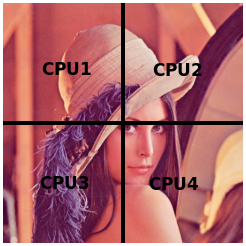
\includegraphics[width=0.3\linewidth]{figs/lenna.png}
	\caption{Subdivisão das imagens.}
	\label{fig:lena}
\end{figure}

Cada processador fica responsável por realizar o algoritmo de conversão em
escala de cinza em uma determinada região da imagem (quando é utilizado
realmente 4 \textit{threads}). Todo esse processo é realizado para cada imagem
até que todas as imagens sejam processadas.
 
